% ycb1-fig-reciprocal-inhibition. Labels from notes block ycb1-hl-human-body-introduction,
% "Reflex and reciprocal inhibition" bullet (checked in pass 4): when one muscle contracts its opposite relaxes
% (biceps and triceps), giving smooth movement.
\documentclass[border=6pt]{standalone}
% Shared preamble for the YCB1 line diagrams (standalone TikZ, XeTeX). Black and white only; labels come from
% the checked notes block named in each diagram file. Build: make_figures.bat in this folder.
\usepackage{fontspec}
\setmainfont{Segoe UI}
\usepackage{tikz}
\usetikzlibrary{arrows.meta,positioning,shapes.geometric,calc,decorations.pathreplacing}
\hyphenpenalty=10000 \exhyphenpenalty=10000 % no hyphenated labels
\tikzset{
  box/.style={draw, rounded corners=2pt, align=center, inner sep=4pt, font=\small, minimum height=1.6em},
  head/.style={box, font=\small\bfseries},
  note/.style={align=center, font=\footnotesize},
  link/.style={-{Stealth[length=2mm]}, thin},
}

\begin{document}
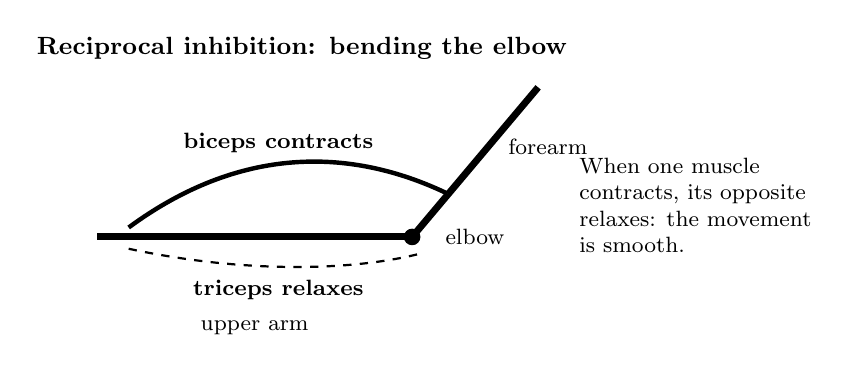
\begin{tikzpicture}
\node[font=\small\bfseries] at (2.6,2.4) {Reciprocal inhibition: bending the elbow};
% upper arm bone and forearm as thick lines, elbow as a joint dot
\draw[line width=2.5pt] (0,0) -- (4,0) node[midway, below=9mm, note] {upper arm};
\draw[line width=2.5pt] (4,0) -- (5.6,1.9) node[pos=0.6, right=1mm, note] {forearm};
\fill (4,0) circle (3pt) node[right=3mm, note] {elbow};
% biceps on top, short and thick (contracts); triceps below, long and thin (relaxes)
\draw[line width=1.6pt, fill=white, rounded corners=6pt] (0.4,0.12) .. controls (1.8,1.15) and (3.2,1.15) .. (4.45,0.55);
\node[note, above] at (2.3,0.95) {\textbf{biceps contracts}};
\draw[dashed, thick] (0.4,-0.15) .. controls (1.8,-0.45) and (3.2,-0.45) .. (4.15,-0.2);
\node[note, below] at (2.3,-0.42) {\textbf{triceps relaxes}};
\node[note, align=left, anchor=west] at (6.0,0.4) {When one muscle\\contracts, its opposite\\relaxes: the movement\\is smooth.};
\end{tikzpicture}
\end{document}
